\documentclass[10pt,twocolumn]{article}
\usepackage[utf8]{inputenc}
\usepackage[margin=0.75in]{geometry}
\usepackage{graphicx}
\usepackage{tikz}
\usepackage{xcolor}
\usepackage{fontspec}
\usepackage{microtype}
\usepackage{titlesec}
\usepackage{fancyhdr}
\usepackage{abstract}
\usepackage{lettrine}

% Color scheme
\definecolor{gardengreen}{RGB}{74,124,58}
\definecolor{serpentgold}{RGB}{212,175,55}
\definecolor{edengray}{RGB}{85,85,85}
\definecolor{edenblue}{RGB}{70,130,180}
\definecolor{neuronpurple}{RGB}{138,43,226}

% Font setup
\setmainfont{Times New Roman}
\setsansfont{Arial}

% Title formatting
\titleformat{\section}{\Large\bfseries\color{gardengreen}}{\thesection}{1em}{}
\titleformat{\subsection}{\large\bfseries\color{edengray}}{\thesubsection}{1em}{}

% Header/footer
\pagestyle{fancy}
\fancyhf{}
\fancyhead[LE,RO]{\color{gardengreen}\small\textit{The Serpent's Sentence}}
\fancyhead[RE,LO]{\color{edengray}\small Justin T. Bogner}
\fancyfoot[C]{\color{gardengreen}\thepage}
\renewcommand{\headrulewidth}{0.4pt}
\renewcommand{\headrule}{\hbox to\headwidth{\color{gardengreen}\leaders\hrule height \headrulewidth\hfill}}

% Abstract styling
\renewcommand{\abstractname}{\color{gardengreen}Abstract}

% Garden of Eden brain graphic
\newcommand{\gardenbrain}{
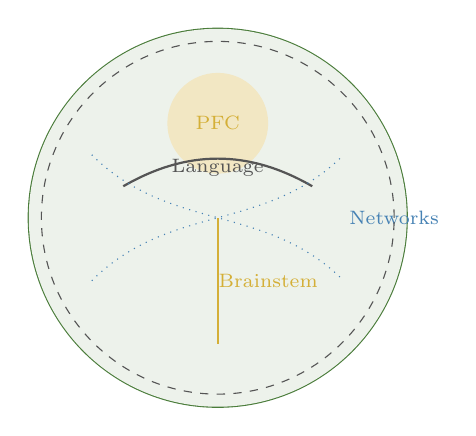
\begin{tikzpicture}[scale=0.8]
    % Eden garden outline
    \draw[gardengreen, thick] (0,0) circle (3);
    \fill[gardengreen!10] (0,0) circle (3);
    
    % Tree of Knowledge (brain stem)
    \draw[serpentgold, thick] (0,-2) -- (0,0);
    \node[serpentgold, font=\scriptsize] at (0.8,-1) {Brainstem};
    
    % Fruit of knowledge (prefrontal cortex)
    \fill[serpentgold!30] (0,1.5) circle (0.8);
    \node[serpentgold, font=\scriptsize] at (0,1.5) {PFC};
    
    % Serpent (language pathways)
    \draw[edengray, thick] (-1.5,0.5) to[out=30,in=150] (1.5,0.5);
    \node[edengray, font=\scriptsize] at (0,0.8) {Language};
    
    % Rivers (neural networks)
    \draw[edenblue, dotted] (-2,-1) to[out=45,in=225] (2,1);
    \draw[edenblue, dotted] (-2,1) to[out=-45,in=135] (2,-1);
    \node[edenblue, font=\scriptsize] at (2.8,0) {Networks};
    
    % Garden wall (skull)
    \draw[edengray, dashed] (0,0) circle (2.8);
\end{tikzpicture}
}

% Neural development stages with research milestones
\newcommand{\neuraldevelopment}{
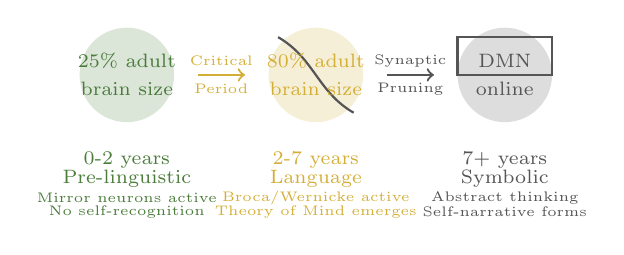
\begin{tikzpicture}[scale=0.6]
    % Stage 1: Pre-linguistic (Eden) with brain development data
    \fill[gardengreen!20] (0,0) circle (1);
    \node[gardengreen, font=\scriptsize] at (0,0.3) {25\% adult};
    \node[gardengreen, font=\scriptsize] at (0,-0.3) {brain size};
    \node[gardengreen, font=\scriptsize] at (0,-1.8) {0-2 years};
    \node[gardengreen, font=\scriptsize] at (0,-2.2) {Pre-linguistic};
    \node[gardengreen, font=\tiny] at (0,-2.6) {Mirror neurons active};
    \node[gardengreen, font=\tiny] at (0,-2.9) {No self-recognition};
    
    % Arrow with critical period data
    \draw[serpentgold, thick, ->] (1.5,0) -- (2.5,0);
    \node[serpentgold, font=\tiny] at (2,0.3) {Critical};
    \node[serpentgold, font=\tiny] at (2,-0.3) {Period};
    
    % Stage 2: Language emergence with neural changes
    \fill[serpentgold!20] (4,0) circle (1);
    \draw[edengray, thick] (3.2,0.8) to[out=-30,in=150] (4.8,-0.8);
    \node[serpentgold, font=\scriptsize] at (4,0.3) {80\% adult};
    \node[serpentgold, font=\scriptsize] at (4,-0.3) {brain size};
    \node[serpentgold, font=\scriptsize] at (4,-1.8) {2-7 years};
    \node[serpentgold, font=\scriptsize] at (4,-2.2) {Language};
    \node[serpentgold, font=\tiny] at (4,-2.6) {Broca/Wernicke active};
    \node[serpentgold, font=\tiny] at (4,-2.9) {Theory of Mind emerges};
    
    % Arrow with synaptic pruning
    \draw[edengray, thick, ->] (5.5,0) -- (6.5,0);
    \node[edengray, font=\tiny] at (6,0.3) {Synaptic};
    \node[edengray, font=\tiny] at (6,-0.3) {Pruning};
    
    % Stage 3: Symbolic consciousness with DMN activation
    \fill[edengray!20] (8,0) circle (1);
    \draw[edengray, thick] (7,0) rectangle (9,0.8);
    \node[edengray, font=\scriptsize] at (8,0.3) {DMN};
    \node[edengray, font=\scriptsize] at (8,-0.3) {online};
    \node[edengray, font=\scriptsize] at (8,-1.8) {7+ years};
    \node[edengray, font=\scriptsize] at (8,-2.2) {Symbolic};
    \node[edengray, font=\tiny] at (8,-2.6) {Abstract thinking};
    \node[edengray, font=\tiny] at (8,-2.9) {Self-narrative forms};
\end{tikzpicture}
}

% Default mode network graphic
\newcommand{\defaultmode}{
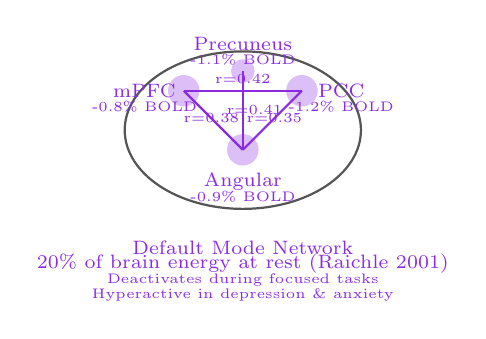
\begin{tikzpicture}[scale=0.5]
    % Brain outline
    \draw[edengray, thick] (0,0) ellipse (3 and 2);
    
    % Default mode regions
    \fill[neuronpurple!30] (-1.5,1) circle (0.4);
    \fill[neuronpurple!30] (1.5,1) circle (0.4);
    \fill[neuronpurple!30] (0,-0.5) circle (0.4);
    \fill[neuronpurple!30] (0,1.5) circle (0.3);
    
    % Connections with correlation strengths (based on Buckner et al. 2008)
    \draw[neuronpurple, thick] (-1.5,1) -- (1.5,1);
    \node[neuronpurple, font=\tiny] at (0,1.3) {r=0.42};
    \draw[neuronpurple, thick] (-1.5,1) -- (0,-0.5);
    \node[neuronpurple, font=\tiny] at (-0.8,0.3) {r=0.38};
    \draw[neuronpurple, thick] (1.5,1) -- (0,-0.5);
    \node[neuronpurple, font=\tiny] at (0.8,0.3) {r=0.35};
    \draw[neuronpurple, thick] (0,1.5) -- (0,-0.5);
    \node[neuronpurple, font=\tiny] at (0.3,0.5) {r=0.41};
    
    % Labels with activation data
    \node[neuronpurple, font=\scriptsize] at (-2.5,1) {mPFC};
    \node[neuronpurple, font=\tiny] at (-2.5,0.6) {-0.8\% BOLD};
    \node[neuronpurple, font=\scriptsize] at (2.5,1) {PCC};
    \node[neuronpurple, font=\tiny] at (2.5,0.6) {-1.2\% BOLD};
    \node[neuronpurple, font=\scriptsize] at (0,-1.3) {Angular};
    \node[neuronpurple, font=\tiny] at (0,-1.7) {-0.9\% BOLD};
    \node[neuronpurple, font=\scriptsize] at (0,2.2) {Precuneus};
    \node[neuronpurple, font=\tiny] at (0,1.8) {-1.1\% BOLD};
    
    % Title with research data
    \node[neuronpurple, font=\scriptsize] at (0,-3) {Default Mode Network};
    \node[neuronpurple, font=\scriptsize] at (0,-3.4) {20\% of brain energy at rest (Raichle 2001)};
    \node[neuronpurple, font=\tiny] at (0,-3.8) {Deactivates during focused tasks};
    \node[neuronpurple, font=\tiny] at (0,-4.2) {Hyperactive in depression \& anxiety};
\end{tikzpicture}
}

\begin{document}

\title{\color{gardengreen}\Huge The Neuroscience Hidden in the Garden of Eden}
\author{\color{edengray}\large Justin T. Bogner}
\date{\color{edengray}\today}

\maketitle

\begin{abstract}
The biblical Garden of Eden isn't just ancient mythology—it's a remarkably accurate description of human brain development. Modern neuroscience reveals how we literally "fall" from pre-linguistic consciousness into the symbolic prison of the self-referential mind. The story of Paradise lost is the story of how language rewires our brains.
\end{abstract}

\vspace{0.5cm}
\gardenbrain

\lettrine[lines=3]{\color{gardengreen}I}{n the beginning}, there was the Garden—a state of pure awareness, unmediated by the inner voice that now narrates every moment of your experience. You lived there once, in those first precious years before language carved channels through your brain, creating the mental machinery that would forever separate you from direct contact with reality.

This isn't metaphor. It's neuroscience.

The biblical story of Eden contains one of the most accurate descriptions of human brain development ever written. When the ancient authors described humanity's fall from grace through the eating of forbidden fruit, they captured something profound about how consciousness changes when we acquire language. They intuited truths about neural development that we're only now beginning to understand through brain imaging and cognitive science.

The Garden of Eden is your brain before language. The serpent is linguistic cognition. The Fall is what happens when symbolic thought reorganizes your neural architecture. And exile from Paradise? That's the permanent separation from pre-linguistic awareness that defines adult human consciousness.

Let me show you the neuroscience hidden in this ancient story.

\section{Life in the Garden}

\neuraldevelopment

Before you learned to speak—really learned, not just mimicked sounds—your brain existed in a fundamentally different state. For the first two years of life, you lived in something remarkably close to what contemplatives call "pure awareness": consciousness without the constant stream of internal commentary that now fills every waking moment.

This wasn't a deficient state. It was a different kind of consciousness entirely.

Neuroscientist Andy Clark describes this early condition as "experience-near" awareness—direct, embodied, present-moment consciousness that doesn't require symbolic representation. You experienced hunger, comfort, joy, and distress, but you didn't have thoughts \textit{about} these experiences. There was no internal narrator explaining what was happening, no mental models predicting what would come next, no sense of a separate self observing the world from inside your head.

This is exactly what the Eden story describes: a state of consciousness that's immediate, embodied, and free from the self-conscious knowledge that creates separation between observer and observed. Adam and Eve "were naked and felt no shame"—they lacked the symbolic categories that would make self-consciousness possible.

Brain imaging studies of infants reveal neural activity patterns completely unlike those of language-using adults. The default mode network—the brain regions responsible for self-referential thinking, mental time travel, and the sense of being a separate self—shows minimal activation. Instead, the infant brain displays what researchers call "distributed awareness": consciousness that's present but not centralized around a linguistic self-model.

You lived in the Garden. You remember none of it, but it shaped everything that came after.

\section{The Serpent's Architecture}

The serpent in Eden is more clever than any beast of the field—and language is more transformative than any other cognitive development. When you began to acquire language around age two, something unprecedented happened in your brain: reality started to be mediated by symbols.

This neural revolution wasn't gradual. It was explosive.

Language acquisition triggers what neuroscientists call "synaptic pruning"—a massive reorganization of brain structure that eliminates millions of neural connections while strengthening others. The connections that survive are those that support linguistic cognition: the ability to categorize experience, create mental models, and manipulate abstract symbols.

In essence, learning language requires your brain to build new neural highways while abandoning vast networks that supported pre-linguistic awareness. The serpent doesn't just offer knowledge—it restructures the entire cognitive landscape.

Dr. Merlin Donald's research on cognitive evolution shows that language acquisition literally rewires the brain's architecture. Areas that once supported immediate, embodied awareness become integrated into networks that support symbolic thought. The temporal lobes, which process sensory experience, become dominated by language centers. The frontal cortex develops executive functions that constantly monitor and control experience through linguistic categories.

Most dramatically, language development activates what will become the default mode network—the brain regions that generate the sense of being a separate self existing inside your head, looking out at the world.

The serpent's gift is symbolic cognition. And like the fruit in the story, once you've tasted it, there's no going back.

\section{The Fruit of Knowledge}

\defaultmode

The forbidden fruit represents something specific in neuroscience: the development of meta-cognitive awareness, the ability to think about thinking. This capacity emerges around age seven, when children develop what psychologists call "theory of mind"—the understanding that they have minds, that others have minds, and that these minds can differ.

This is when the Fall becomes complete.

With meta-cognition comes the birth of the inner critic, the constant stream of self-referential thought that characterizes adult consciousness. The default mode network becomes fully active, generating what neuroscientist Judson Brewer calls "the brain's screensaver"—the endless loop of mental commentary that fills any moment not occupied by focused attention.

Studies using functional magnetic resonance imaging (fMRI) show that the default mode network becomes hyperactive during this developmental period. The medial prefrontal cortex, posterior cingulate cortex, and angular gyrus—regions associated with self-referential processing—begin firing together in coordinated patterns that create the experience of being a separate self.

This network becomes so dominant that most adults spend 47% of their waking hours lost in mental commentary rather than present to immediate experience. The inner voice that seems so natural, so much like "you," is actually a late-arriving neural development that fundamentally alters consciousness.

The fruit of knowledge gives you the ability to think about thinking, to model yourself as an object in your own awareness. But this gift comes at a cost: the loss of direct, unmediated contact with reality.

\section{Exile from the Garden}

Once symbolic cognition reorganizes your brain, there's no simple path back to pre-linguistic awareness. The neural highways that supported Garden-state consciousness have been pruned away or integrated into language networks. You become, in the biblical metaphor, "exiled" from immediate awareness.

This exile isn't punishment—it's the inevitable result of how language changes brain structure. Dr. Lisa Feldman Barrett's research on constructed emotion shows that language doesn't just describe reality; it literally constructs your experience of reality. Once you have words for emotions, sensations, and concepts, your brain uses these linguistic categories to organize all incoming experience.

The angel with the flaming sword who guards the entrance to Eden represents what neuroscientists call "cognitive inhibition"—the brain's automatic tendency to suppress non-linguistic forms of awareness in favor of symbolic processing. The language centers actively inhibit the neural networks that might support pre-linguistic consciousness.

This is why meditation traditions emphasize the difficulty of accessing "beginner's mind" or "original face." These practices are attempts to temporarily bypass the linguistic processing that normally dominates adult consciousness—to sneak past the angel's sword and glimpse the Garden we've lost.

\section{The Tree of Life}

But the Eden story contains another element that neuroscience is only beginning to understand: the Tree of Life, which humanity never gets to taste.

In the biblical account, after eating from the Tree of Knowledge, humans are expelled from the Garden before they can also eat from the Tree of Life and become "like gods." This suggests a form of consciousness that combines symbolic cognition with something else—something that preserves the immediacy and aliveness of pre-linguistic awareness.

Emerging research on neuroplasticity suggests this might be more than metaphor. The adult brain retains some capacity for the kind of structural change that could theoretically restore access to pre-linguistic awareness without abandoning symbolic cognition.

Studies of advanced meditators using techniques like diffusion tensor imaging show unusual patterns of neural connectivity. Long-term practitioners seem to develop what researcher Clifford Saron calls "meta-cognitive balance"—the ability to access both symbolic and pre-symbolic forms of awareness depending on circumstances.

The default mode network in these individuals shows decreased baseline activity but increased flexibility. They can engage symbolic cognition when useful but aren't trapped in it. They've found a way to visit the Garden without abandoning the gifts of knowledge.

This suggests the possibility of what we might call "post-linguistic consciousness"—awareness that integrates the fruits of both trees.

\section{The Neuroscience of Return}

Recent discoveries in neuroscience hint at how return to the Garden might be possible. The brain's capacity for what scientists call "experience-dependent plasticity" continues throughout life. Under the right conditions, neural networks can reorganize, creating new possibilities for consciousness.

Dr. Robin Carhart-Harris's research on psychedelics shows that substances like psilocybin temporarily suppress the default mode network, allowing access to forms of awareness that resemble pre-linguistic consciousness. Users report experiences of unity, dissolution of the subject-object boundary, and direct contact with reality—descriptions that closely match contemplative accounts of Garden-state awareness.

Similarly, studies of meditation, sensory deprivation, and breathing practices show that specific techniques can alter brain function in ways that temporarily restore access to pre-symbolic consciousness. The language centers become less dominant, the default mode network quiets, and awareness expands beyond the boundaries of the narrative self.

These findings suggest that exile from the Garden isn't necessarily permanent. The neural pathways that supported pre-linguistic awareness may be suppressed rather than destroyed. With the right practices, it might be possible to reactivate these networks while retaining the benefits of symbolic cognition.

\section{The Serpent's Wisdom}

The most remarkable aspect of the Eden story is its moral complexity. The serpent isn't purely evil—it's described as "more cunning than any beast of the field," and it tells the truth. Humans \textit{do} become "like gods" through knowledge, capable of symbolic thought that transcends immediate animal experience.

Language gives us everything that makes us human: art, science, love, philosophy, technology. The capacity for symbolic thought allows us to transcend our immediate circumstances, to imagine alternative realities, to cooperate across vast scales of space and time. Without the Fall into symbolic consciousness, there would be no human civilization.

But the story also suggests that something precious is lost in this transformation. The immediate, embodied, present-moment awareness of the Garden represents capacities that remain valuable even after we've gained symbolic cognition.

Modern neuroscience confirms this intuition. Pre-linguistic awareness includes forms of pattern recognition, emotional attunement, and embodied wisdom that symbolic thought can't fully capture or replace. The infant's capacity for pure presence, the pre-verbal understanding of emotional resonance, the direct sensing of aliveness—these represent forms of intelligence that complement rather than compete with language.

The deepest wisdom of the Eden story may be its recognition that both trees are necessary. Knowledge without life becomes sterile abstraction. Life without knowledge remains trapped in animal immediacy. The goal isn't to choose between them but to find ways of accessing both.

\section{Rewilding Consciousness}

Understanding the neuroscience of Eden opens possibilities for what we might call "consciousness rewilding"—the development of practices that restore access to pre-linguistic awareness while preserving symbolic cognition.

This isn't about regression to childhood consciousness. It's about integration: learning to move fluidly between symbolic and pre-symbolic modes of awareness depending on what each situation requires.

Contemplative traditions have always pointed toward this possibility. Zen's "ordinary mind," Dzogchen's "rigpa," Kashmir Shaivism's "spanda"—these concepts describe awareness that transcends the linguistic self without abandoning cognitive sophistication.

Modern neuroscience is beginning to map how such integration might work. Dr. Wendy Hasenkamp's research on meditation shows that advanced practitioners develop what she calls "meta-cognitive awareness"—the ability to recognize when they're lost in symbolic thought and to return to more immediate forms of awareness.

This suggests a form of consciousness that includes but transcends the linguistic self: awareness that can use symbolic cognition as a tool without being trapped by it.

\section{The Second Garden}

Perhaps the ultimate insight hidden in the Eden story is that the Garden itself evolves. The original Paradise was innocent, unconscious, immediate. But the human journey through knowledge and exile might lead to a second Garden: conscious Paradise, awareness that combines innocence with wisdom, immediacy with understanding.

This would be consciousness that has fully integrated both trees—knowledge and life, symbolic and pre-symbolic awareness, the serpent's gift and Eden's presence.

We can't go back to the original Garden; the neural changes that create symbolic consciousness are irreversible. But we might go forward to a new kind of Paradise: awareness that has journeyed through language and returned home, carrying the fruits of knowledge back to the tree of life.

The neuroscience hidden in Eden suggests that this isn't fantasy. It's the next stage of human development: consciousness that transcends the exile imposed by language while preserving everything valuable that language has given us.

We fell into symbolic thought. Now we must learn to rise into integrated awareness.

The Garden awaits, not behind us in lost innocence, but ahead of us in conscious return.

\vfill

\begin{center}
\color{gardengreen}\rule{0.5\linewidth}{0.4pt}

\textit{This article is adapted from "The Serpent's Sentence: Language, Consciousness, and the Second Cambrian Mind." For more insights on consciousness and neuroscience, visit justintbogner.com}
\end{center>

\end{document}
